\documentclass[english]{article}
\usepackage{graphicx}
\usepackage[margin=.8in]{geometry}
\usepackage{float}
\usepackage{hyperref}
\hypersetup{
    colorlinks=true,
    linkcolor=blue,
    filecolor=blue,      
    urlcolor=blue,
}

\begin{document}

\title{ User Manual \\
	\large For Pascal to Mips Compiler}
\author{Joseph Miller}
\maketitle

\section{Using the compiler} \label{using}

Below is a series of steps in order to take your Pascal code and create MIPs assembly code.

\begin{enumerate}
   \item Open the command prompt or terminal on your computer
   \item Navigate to the directory that contains Compiler.jar
   \item Enter the following into the command line: \textbf{java -jar Compiler.jar pascalfile.pas}
\end{enumerate}

\noindent There should be three new files in the directory that Compiler.jar was run in. If not, reference section \ref{errors}

\begin{itemize}
   \item  \textit{pascalfilename.asm} : the compiled assembly code
   \item  \textit{pascalfilename.table} : the symbol table of variables declared
   \item  \textit{pascalfilename.tree}: syntax tree of the pascal code
\end{itemize}

\noindent The .asm can be run in \href{http://spimsimulator.sourceforge.net/}{QtSpim} - a simulator for MIPs assembly code. The interface can be seen below.

\begin{figure}[H]
\begin{center}
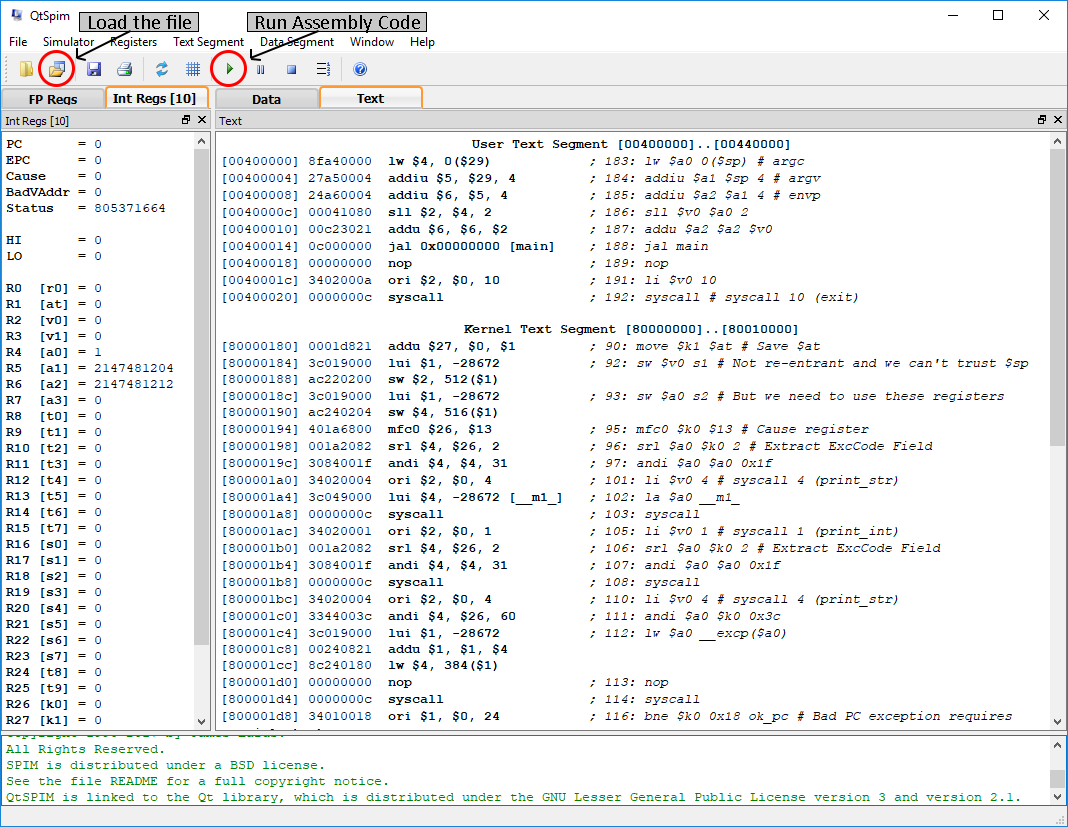
\includegraphics[width=.8\textwidth]{qtspim.PNG}
\end{center}
\caption{\label{QtSpim}QtSpim Interface}
\end{figure}


\section{Error Handling} \label{errors}

\subsection{Match of a different token then expected} \label{tokenerror}

If you've received an error such as "Error Match of END found SEMI instead." this means that the pascal code was invalid and not a proper sequence of tokens. Reevaluate the Pascal code and check for extra or missing semi-colons. If still no success, review proper Pascal code, this resource may be helpful:  \href{https://en.wikipedia.org/wiki/Pascal_(programming_language)}{Pascal Language}.

\subsection{Error in a grammar  rule}

If you've recieved a message that there has been in error in the following functions in the form "Error in [function name]" then the code is not proper Pascal, most likely an expression or content of a statement. Refer back to section \ref{tokenerror}
\begin{itemize}
   \item "Error in factor"
   \item "Error in mulop"
   \item "Error in simple expression"
\end{itemize}

\subsection{Command prompt / terminal cannot find 'java' command}

If your command prompt or terminal doesn't recognize the command 'java' then either java is not installed on your system of it isn't set in your environment variables. This link can help if you don't have java installed:   \href{https://www.java.com/en/download/help/download_options.xml}{Installing Java}. This link may help to set Java as a system variable:   \href{https://www.java.com/en/download/help/path.xmll}{Set or change system variables}


\subsection{Code compiles but does not run in QtSpim}

If your code compiles properly (e.i. you generate the three files referenced in section \ref{using}) but QtSpim can't properly handle it then most likely the code is proper Pascal but doesn't make sense logically. Carefully  review the code and try and identify any logical errors that may have occurred  - such as infinite  loops or impossible conditions.






\end{document}